\documentclass[11pt,aspectratio=169]{beamer}

% Encoding and language
\usepackage[utf8]{inputenc} % encoding
\usepackage[T1]{fontenc} % PostScript font
\usepackage[english]{babel} % English text
\usepackage{datetime} % date

% Useful packages
\usepackage{amsmath, amsthm} % mathematical mode
\usepackage{amsfonts,amssymb} % definition of sets
\usepackage{graphicx} % image management
\usepackage{float} % figure placement
\usepackage{hyperref} % clickable link management
\usepackage{url} % URL management
\usepackage{listings} % display code
\usepackage{xcolor} % color management
\usepackage{caption} % better legends
\usepackage{verbatim} % special character handling
\usepackage{textcomp} % adds special characters (like ¥)
\usepackage{tikz} % flowcharts and graphs
\usetikzlibrary{shapes.geometric, arrows.meta, positioning, calc}

% [trim={left bottom right top},clip]

% Define Flowchart Styles
\tikzset{
  startstop/.style={rectangle, rounded corners, minimum width=3cm, minimum height=1cm, text centered, draw=black, fill=red!30},
  process/.style={rectangle, minimum width=3.5cm, minimum height=1cm, text centered, draw=black, fill=orange!30, font=\footnotesize},
  decision/.style={diamond, minimum width=3cm, minimum height=1cm, text centered, draw=black, fill=green!30, font=\footnotesize, aspect=2},
  arrow/.style={thick,->,>=stealth},
  connector/.style={draw, -latex, thick}
}

% Color definition
\definecolor{yamlkeyword}{rgb}{0.5, 0.0, 0.5} % YAML keywords (true, false, null)
\definecolor{yamlcomment}{rgb}{0.4, 0.4, 0.4} % YAML comments (#)
\definecolor{yamldelimiter}{rgb}{0.8, 0.0, 0.0} % YAML delimiter (:)
\definecolor{yamlstring}{rgb}{0.1, 0.1, 0.9} % YAML strings

\definecolor{pykeyword}{rgb}{0.0, 0.5, 0.0} % Python keywords
\definecolor{pycomment}{rgb}{0.2, 0.4, 0.6} % Python comments
\definecolor{pystring}{rgb}{0.8, 0.3, 0.1} % Python strings

\definecolor{bashkeyword}{rgb}{0.1, 0.5, 0.5} % Commands like 'if', 'for', 'echo'
\definecolor{bashcomment}{rgb}{0.2, 0.4, 0.6} % Comments (#)
\definecolor{bashstring}{rgb}{0.8, 0.3, 0.1} % Strings (text between quotes)
\definecolor{bashvariable}{rgb}{0.9, 0.4, 0.0} % Variables ($VAR)

% Common listing style configuration
\lstdefinestyle{codestyle}{
  basicstyle=\ttfamily\tiny, % text size
  numbers=left,
  numberstyle=\tiny\color{gray},
  stepnumber=1,
  numbersep=5pt,
  frame=single,
  framerule=0.5pt,
  tabsize=2,
  showstringspaces=false,
  breaklines=true,
  captionpos=b,
  keepspaces=true
}

% YAML style configuration
\lstdefinelanguage{yaml}{ % YAML is not a language included in listing
  keywords={true, false, null, y, n},
  keywordstyle=\color{yamlkeyword}\bfseries,
  comment=[l]{\#},
  commentstyle=\color{yamlcomment}\ttfamily,
  stringstyle=\color{yamlstring}\ttfamily,
  literate={:}{{{\color{yamldelimiter}:}}}1
}
\lstdefinestyle{yamlstyle}{
  style=codestyle,
  language=yaml,
  tabsize=2
}

% Python style configuration
\lstdefinestyle{pythonstyle}{
  style=codestyle,
  language=Python,
  tabsize=4,
  identifierstyle=\color{black},
  commentstyle=\color{pycomment}\ttfamily,
  keywordstyle=\color{pykeyword}\bfseries,
  stringstyle=\color{pystring}
}

% --- Bash style configuration ---
\lstdefinestyle{bashstyle}{
  style=codestyle,
  language=bash, % Use 'bash' or 'sh' for shell scripts
  tabsize=4,
  identifierstyle=\color{black},
  commentstyle=\color{bashcomment}\ttfamily,
  keywordstyle=\color{bashkeyword}\bfseries,
  stringstyle=\color{bashstring},
  morekeywords={ls, cd, pwd, echo, grep, awk, sed, exit, source, export, read}, % Common commands
  alsoother={\$}, % Treat '$' as part of an identifier to highlight variables
  literate={-}{-}1, % Ensures proper rendering of dashes
  literate={\$}{{{\color{bashvariable}\$}}}1
           {VAR}{{{\color{bashvariable}VAR}}}1
           {FILE}{{{\color{bashvariable}FILE}}}1
           {¥}{{{\textyen}}}1 % replaces the character ¥ with the LaTeX command \textyen
}

\usetheme{Ilmenau} % presentation theme

\setlength{\fboxsep}{0.8pt} % image outline thickness
\newcommand{\blueframeimg}[2][]{%
  \fcolorbox{blue}{blue}{\includegraphics[#1]{#2}}%
}

\addtobeamertemplate{footline}{
  \hspace{0.1cm}
  \footnotesize
  \insertframenumber/\inserttotalframenumber
} % number of slides

% Presentation cover
\title{Graph-based Expense Optimization}
\subtitle{Graphs and Applications}
\author{Jacopo \& Mathis}
\institute{Tongji University}
\newdate{date}{17}{12}{2025}
\date{\displaydate{date}}
\titlegraphic{\includegraphics[width=0.1\textwidth]{img/tongji.png}}

\begin{document}

% Presentation cover
\frame{\titlepage}

% Introduction
\begin{frame}[plain] % The [plain] option removes the headers/footers
\centering
\begin{tabular}{cc}
  \onslide<1->{
    \begin{minipage}{0.35\textwidth}
    \blueframeimg[width=\textwidth]{img/img1.png}
    \end{minipage}
  } &
  \onslide<2->{
    \begin{minipage}{0.35\textwidth}
    \blueframeimg[width=\textwidth]{img/img2.png}
    \end{minipage}
  } \\[2cm]

  \onslide<3->{
    \begin{minipage}{0.35\textwidth}
    \blueframeimg[width=\textwidth]{img/img3.png}
    \end{minipage}
  } &
  \onslide<4->{
    \begin{minipage}{0.35\textwidth}
    \includegraphics[width=\textwidth]{img/tricount-1.png}
    \end{minipage}
  } \\
\end{tabular}
\end{frame}

% Table of contents
\begin{frame}{Outline}
  \tableofcontents
\end{frame}

% ==========================================
% SECTION 1: CONTEXT
% ==========================================
\section{What is Tricount?}
\begin{frame}{What is Tricount?}
  \begin{block}{}
    Tricount is a collaborative application designed to simplify expense sharing among groups, such as roommates or travelers.
  \end{block}
  \begin{columns}[T]
    \begin{column}{0.6\textwidth}
      \begin{block}<2->{}
        \begin{itemize}
          \item<2-> \textbf{Expense logging:} Users record shared costs, specifying who paid and who benefited.
          \item<3-> \textbf{Balance calculation:} It computes the net balance to see who is in debt and who is a creditor.
          \item<4-> \textbf{Transaction optimization:} It calculates the minimum transfers needed to settle all debts.
        \end{itemize}
      \end{block}
    \end{column}
    \begin{column}{0.3\textwidth}
      \includegraphics[width=\textwidth,trim={60 60 60 60},clip]{img/tricount-2.png}
    \end{column}
  \end{columns}
\end{frame}

\begin{frame}{Alternative to Tricount}
  \begin{block}{}
    This presentation is not sponsored by Tricount\\
    Here are some equivalent tools:
  \end{block}
  \vspace{0.5cm}
  \begin{columns}[T]
  \begin{column}{0.5\textwidth}
    \includegraphics[width=\textwidth,trim={0 0 0 0},clip]{img/splitwise.png}
  \end{column}
  \begin{column}{0.5\textwidth}
    \includegraphics[width=\textwidth,trim={0 0 0 0},clip]{img/splid.png}
  \end{column}
\end{columns}
\end{frame}

% ==========================================
% SECTION 2: MODELING
% ==========================================
\section{Modeling the problem}
\begin{frame}{Modeling using a graph}
  \begin{block}<1->{Graph representation}
    Based on graph theory definitions, we model the group expenses as a \textbf{directed weighted graph} $D=(V,A)$:
    \begin{itemize}
      \item \textbf{Vertices ($V$):} The set of participants.
      \item \textbf{Arcs ($A$):} The transactions, an arc $(u,v)$ exists if $u$ \textbf{owes} money to $v$.
      \item \textbf{Weight function ($w$):} $w(u, v)$ represents the amount of the debt.
    \end{itemize}
  \end{block}
  \begin{block}<2->{Matrix representation}
    To store the graph, we use an \textbf{adjacency matrix} $M$, where $M_{ij}$ is the \textbf{debt} node $i$ \textbf{owes} node $j$.
  \end{block}
\end{frame}

% ==========================================
% SECTION 3: OPTIMIZATION
% ==========================================
\section{Graph optimization}
\begin{frame}{Calculating balances}
  To simplify the graph, we first calculate the \textbf{net balance} for each vertex.\\
  \begin{block}<2->{Net balance equation}
    For any participant $v \in V$:
    $$\text{Balance}(v)=\underbrace{\sum_{u \in V}w(u,v)}_{\text{in-flow (receivables)}}-\underbrace{\sum_{u \in V}w(v,u)}_{\text{out-flow (payables)}}$$
  \end{block}
  \begin{itemize}
    \item<3-> If $\text{Balance}(v)>0$: $v$ is a \textbf{creditor}
    \item<3-> If $\text{Balance}(v)<0$: $v$ is a \textbf{debtor}
    \item<3-> $\sum_{v \in V}\text{Balance}(v)=0$ (conservation of money)
  \end{itemize}
\end{frame}

\begin{frame}{Reducing transactions}
  \begin{columns}[T]
    \begin{column}{0.55\textwidth}
      \begin{block}{The problem}
        The initial graph often contains redundant cycles (e.g. A owes B, B owes C, C owes A).\\
        We want to construct a new graph $D'$ with the \textbf{minimum number of edges} such that the net balances remain unchanged.
      \end{block}
    \end{column}
    \begin{column}{0.45\textwidth}
      \centering
      \begin{figure}[h]
        \includegraphics[width=\textwidth,trim={10 10 10 10},clip]{img/img15.png}
        \caption{Initial graph}
      \end{figure}
    \end{column}
  \end{columns}
\end{frame}

\begin{frame}{Optimization algorithm (greedy approach)}
  To solve this problem we use a \textbf{greedy algorithm} to resolve the debts.\\
  Greedy algorithms make \textbf{locally optimal} choices at each step with the hope of finding a \textbf{global optimum} solution.
  \begin{block}<2->{}
    \begin{enumerate}
      \item<2-> \textbf{Partition:} Separate vertices into two lists:
      \begin{itemize}
        \item $D$: Debtors (sorted by magnitude of debt descending).
        \item $C$: Creditors (sorted by magnitude of credit descending).
      \end{itemize}
      \item<3-> \textbf{Iterate:} While both lists are non-empty:
      \begin{itemize}
        \item Take the largest debtor $d_{max}$ and largest creditor $c_{max}$.
        \item Amount to transfer: $x=\min(|Balance(d_{max})|,Balance(c_{max}))$.
        \item Create edge $(d_{max},c_{max})$ with weight $x$.
        \item Update balances. If a balance becomes 0, remove from list.
      \end{itemize}
    \end{enumerate}
  \end{block}
  \vspace{0.2cm}
  \only<3->{This approach ensures that at least one participant is settled per transaction.}
\end{frame}

\begin{frame}{Algorithm flowchart}
  \begin{columns}[T]
    \begin{column}{0.6\textwidth}
      \centering
      \resizebox{!}{0.85\textheight}{% fit to height instead of width to prevent overflow
        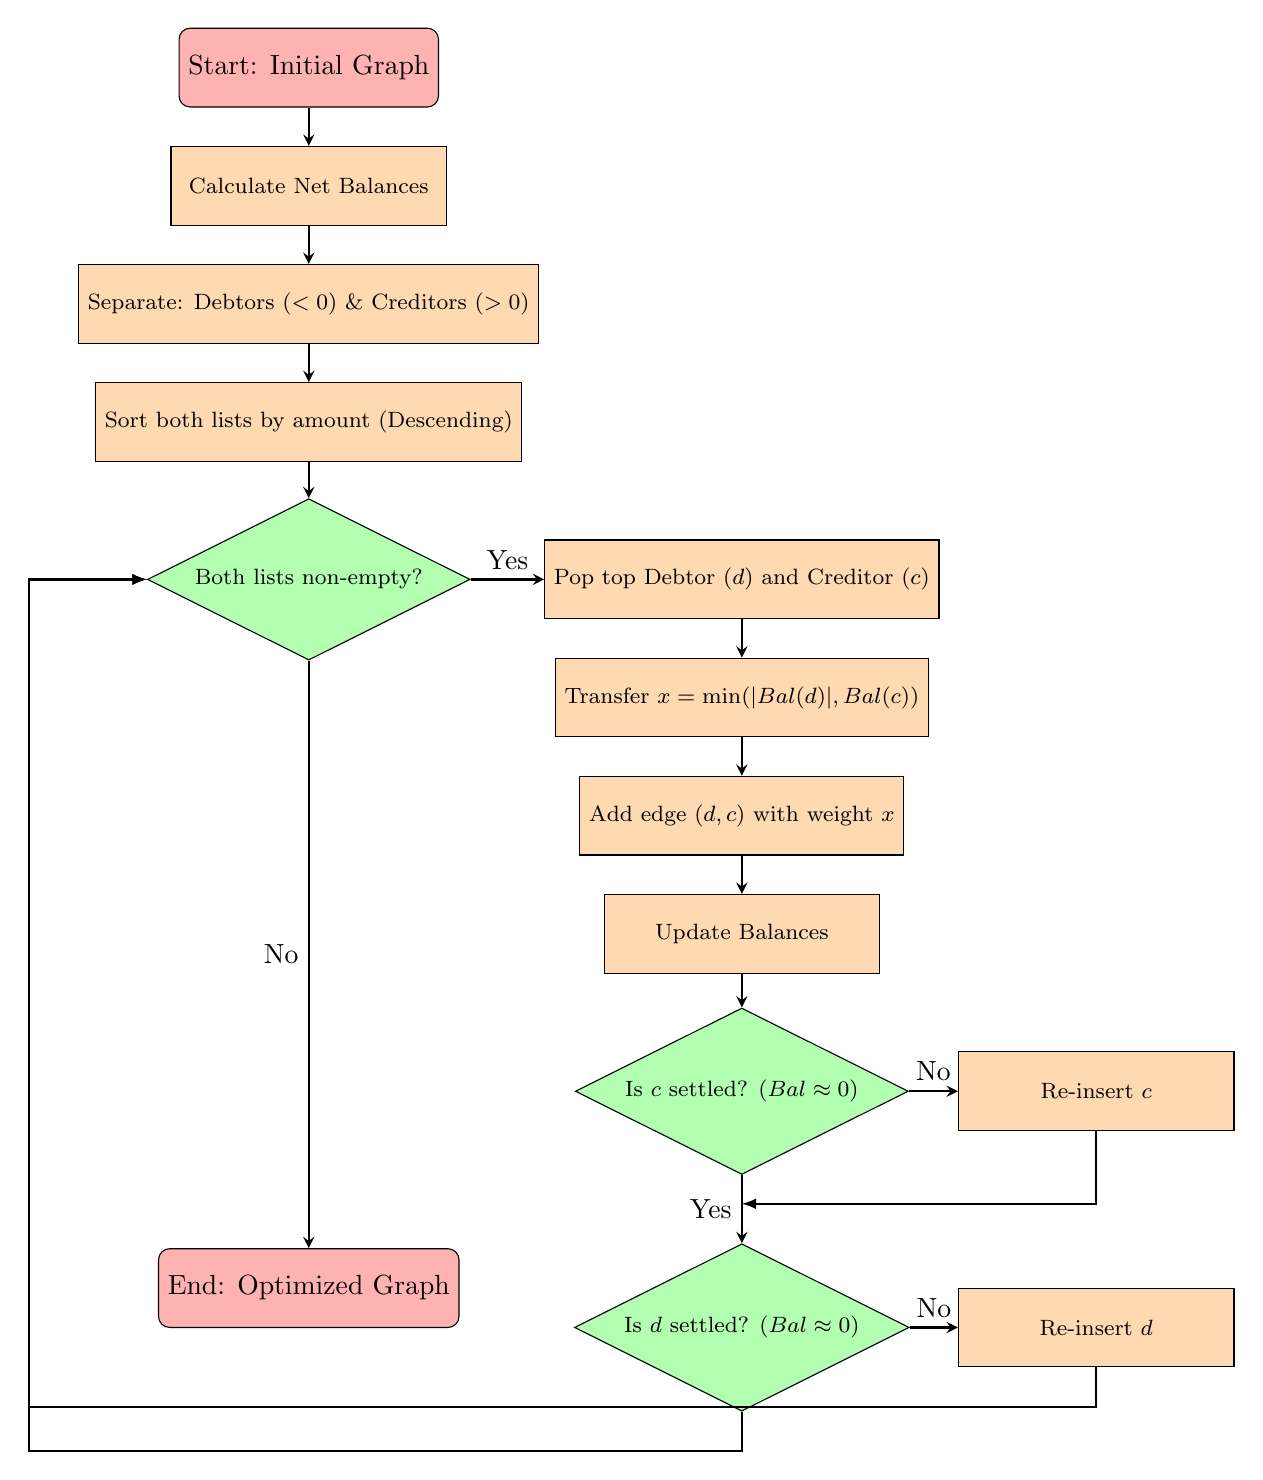
\begin{tikzpicture}[node distance=1.5cm]
        % Nodes
        \node (start) [startstop] {Start: Initial Graph};
        \node (calc_balances) [process, below of=start] {Calculate Net Balances};
        \node (separate_lists) [process, below of=calc_balances] {Separate: Debtors ($<0$) \& Creditors ($>0$)};
        \node (sort_lists) [process, below of=separate_lists] {Sort both lists by amount (Descending)};
        \node (loop_check) [decision, below of=sort_lists, yshift=-0.5cm] {Both lists non-empty?};

        \node (pop_participants) [process, right of=loop_check, xshift=4cm] {Pop top Debtor ($d$) and Creditor ($c$)};
        \node (calc_amount) [process, below of=pop_participants] {Transfer $x = \min(|Bal(d)|, Bal(c))$};
        \node (add_edge) [process, below of=calc_amount] {Add edge $(d, c)$ with weight $x$};
        \node (update_balances) [process, below of=add_edge] {Update Balances};

        \node (check_creditor) [decision, below of=update_balances, yshift=-0.5cm] {Is $c$ settled? ($Bal \approx 0$)};
        \node (reinsert_creditor) [process, right of=check_creditor, xshift=3cm] {Re-insert $c$};

        \node (check_debtor) [decision, below of=check_creditor, yshift=-1.5cm] {Is $d$ settled? ($Bal \approx 0$)};
        \node (reinsert_debtor) [process, right of=check_debtor, xshift=3cm] {Re-insert $d$};

        \node (end) [startstop, below of=loop_check, yshift=-7.5cm] {End: Optimized Graph};

        % Paths
        \draw [arrow] (start) -- (calc_balances);
        \draw [arrow] (calc_balances) -- (separate_lists);
        \draw [arrow] (separate_lists) -- (sort_lists);
        \draw [arrow] (sort_lists) -- (loop_check);

        % Loop Logic
        \draw [arrow] (loop_check.east) -- node[anchor=south] {Yes} (pop_participants.west);
        \draw [arrow] (pop_participants) -- (calc_amount);
        \draw [arrow] (calc_amount) -- (add_edge);
        \draw [arrow] (add_edge) -- (update_balances);
        \draw [arrow] (update_balances) -- (check_creditor);

        % Re-insertion Logic
        \draw [arrow] (check_creditor.east) -- node[anchor=south] {No} (reinsert_creditor.west);
        \draw [arrow] (check_creditor.south) -- node[anchor=east] {Yes} (check_debtor.north);
        \draw [connector] (reinsert_creditor.south) |- ($(check_debtor.north)+(0,0.5)$);

        \draw [arrow] (check_debtor.east) -- node[anchor=south] {No} (reinsert_debtor.west);
        
        % Return paths
        \draw [connector] (check_debtor.south) -- ($(check_debtor.south)-(0,0.5)$) -| ($(loop_check.west)-(1.5,0)$) -- (loop_check.west);
        \draw [connector] (reinsert_debtor.south) -- ($(reinsert_debtor.south)-(0,0.5)$) -| ($(loop_check.west)-(1.5,0)$) -- (loop_check.west);

        \draw [arrow] (loop_check.south) -- node[anchor=east] {No} (end.north);
        \end{tikzpicture}
      }
    \end{column}
    \begin{column}{0.4\textwidth}
      \centering
      \begin{figure}[h]
        \includegraphics[width=1.2\textwidth,trim={200 80 80 80},clip]{img/img16.png}
        \caption{Optimization result}
      \end{figure}
      % \scriptsize
      % \textbf{Trace for Graph (A, B, C):}
      % \begin{itemize}
      %   \setlength\itemsep{0em} % Tighten vertical spacing
      %   \item \textbf{1. Net Balances:}
      %   \begin{itemize}
      %       \scriptsize 
      %       \item A: $1 (\text{in}) - 3 (\text{out}) = \mathbf{-2}$ (Debtor)
      %       \item B: $3 - 4 = \mathbf{-1}$ (Debtor)
      %       \item C: $4 - 1 = \mathbf{+3}$ (Creditor)
      %   \end{itemize}
      %   \item \textbf{2. Sort:} $D=[A, B]$, $C=[C]$.
      %   \item \textbf{3. Match:} Top Debtor ($A$) \& Top Creditor ($C$).
      %   \item \textbf{4. Transfer:} $\min(|-2|, 3) = \mathbf{2}$.
      %   \item \textbf{5. Result:} Edge $A \xrightarrow{2euro} C$ created.
      % \end{itemize}
    \end{column}
  \end{columns}
\end{frame}

% ==========================================
% SECTION 4: DEMONSTRATION
% ==========================================
\section{Demonstration with Graph3Count}
\begin{frame}{Demonstration with Graph3Count}
  \begin{columns}[T]
    \begin{column}<1->{0.6\textwidth}
      \blueframeimg[width=\textwidth,trim={300 0 300 0},clip]{img/img7.png}
    \end{column}
    \begin{column}<2->{0.4\textwidth}
      \begin{tabular}{ccc}
        \includegraphics[width=0.25\linewidth]{img/python.png} &
        \includegraphics[width=0.25\linewidth]{img/yaml.png} &
        \includegraphics[width=0.25\linewidth]{img/json.png} \\[0.3cm]
        \includegraphics[width=0.25\linewidth]{img/html.png} &
        \includegraphics[width=0.25\linewidth]{img/css.png} &
        \includegraphics[width=0.25\linewidth]{img/js.png} \\[0.3cm]
        \includegraphics[width=0.25\linewidth]{img/docker.png} &
        \includegraphics[width=0.25\linewidth]{img/github.png} &
        \includegraphics[width=0.25\linewidth]{img/tex.png} \\
      \end{tabular}
    \end{column}
  \end{columns}
\end{frame}

\begin{frame}[fragile]{How use it?}
  \begin{block}{}
    The \texttt{intent.yaml} file allows you to record the list of participants and the expenses.\\
    It is the entry point between the user and the project.
  \end{block}
  \begin{lstlisting}[style=yamlstyle, caption={\texttt{intent.template.yaml} file}]
members: # list of members (note: if a transaction exists with a member who is not listed here, there is an error)
  - Name 1
  - Name 2
  - Name 3

transactions: # list of transactions (note: you can copy and paste the first dash to add a transaction)
  - from: Name 1 # transaction issuer
    to: # receiver(s) name
      - Name 2
      - Name 3
    amount: 10 # transaction amount (positive if it's an expense, negative if it's an income)
    name: transaction name # transaction name (optional)
    date: YYYY-MM-DD # transaction date (optional)\end{lstlisting}
\end{frame}

\begin{frame}{Web interface}
  \centering
  \includegraphics[width=0.75\textwidth]{img/img8.png}
\end{frame}

\begin{frame}[fragile]{Data structure (\texttt{data.json})}
  \begin{block}{}
    The \texttt{data.json} file stores the graph's adjacency matrix and node names.\\
    Used by backend and frontend.
  \end{block}
  \begin{columns}[T]
    \begin{column}{0.5\textwidth}
      \begin{block}{Structure of  names}
        \scriptsize
        \begin{verbatim}
nodes = [{ "id": 0, "name": "Sarah" },
        { "id": 1, "name": "Jack" },
        { "id": 2, "name": "Victoria" },
        ...
        { "id": n, "name": "James" }]
        \end{verbatim}
      \end{block}
    \end{column}
    \begin{column}{0.5\textwidth}
      \begin{block}{Matrix structure}
        \scriptsize
        \begin{verbatim}
matrix = [[0, 34.9, 51.4, 10.9, ...],
          [60.2, 0, 26.1, 5, ...],
          [6.5, 29.4, 0, 18.2, ...],
          ...
          [45.8, 22.7, 78.2, ..., 0]]
        \end{verbatim}
      \end{block}
    \end{column}
  \end{columns}
\end{frame}

\begin{frame}[fragile]{Code structure}
  \begin{block}{}
    Initializes the graph from data, builds from intent, and optimizes.
  \end{block}
  \begin{lstlisting}[style=pythonstyle, caption={\texttt{main.py} file}]
if __name__ == "__main__":
    print("\nVisit http://localhost:8080/")

    g = Graph("./data/data.json") # Graph creation
    print("\nGraph created")

    process_transactions(g, "./data/intent.example.yaml") # graph construction

    graph_optimization(g)

    #print(g) # for debugging\end{lstlisting}
\end{frame}

\begin{frame}[fragile]{Example (fictional) involving a trip between students}
  \begin{columns}[T]
    \begin{column}<1->{0.45\textwidth}
      \centering
      \begin{block}{}
        Let's imagine four students (Elena, Jacopo, Marco, Mathis) who make 14 transactions during their trip to Beijing
      \end{block}
      \vspace{0.2cm}
      \blueframeimg[width=0.8\textwidth]{img/img9.png}
    \end{column}
    \begin{column}<2->{0.2\textwidth}
      \includegraphics[width=\textwidth]{img/img10.png}
    \end{column}
    \begin{column}<3->{0.3\textwidth}
      \begin{lstlisting}[style=yamlstyle, caption={\texttt{intent.example.yaml} file}]
members:
  - Elena
  - Jacopo
  - Marco
  - Mathis

transactions:
  - from: Jacopo
    to:
      - Elena   
      - Jacopo
      - Marco
      - Mathis
    amount: 70
    name: Return DiDi
    date: 2025-10-18

  - ...\end{lstlisting}
    \end{column}
  \end{columns}
\end{frame}

\begin{frame}[fragile]{Function to create the graph}
  \begin{lstlisting}[style=pythonstyle, caption={\texttt{main.py} file}]
def process_transactions(graph, yaml_path="intent.yaml"):
    with open(yaml_path, "r") as f:
        intent = yaml.safe_load(f)
    
    for member in intent.get("members", []): # add all members
        graph.add_node(member)

    for txn in intent.get("transactions", []): # handle transactions
        sender = txn["from"]
        receivers = txn["to"]
        amount = txn["amount"]

        if not isinstance(receivers, list): # normalize receivers list
            receivers = [receivers]

        if receivers: # split amount equally among receivers
            share = amount / len(receivers)
            for receiver in receivers:
                graph.add_edge(sender, receiver, share)
    
    g.save() # saving the graph to the data.json file\end{lstlisting}
\end{frame}

\begin{frame}{Graph before optimization}
  \begin{figure}[h]
    \includegraphics[width=0.7\textwidth]{img/img11.png}
  \end{figure}
\end{frame}

\begin{frame}[fragile]{Balances calculates}
  \begin{lstlisting}[style=pythonstyle, caption={\texttt{graph.py} file}]
def calculate_net_balances(self):
        '''Calculate the net balance of each member (receivables - payables).'''
        num_nodes = len(self.nodes)
        balances = {}
        for i in range(num_nodes):
            name = self.nodes[i]["name"]

            total_debts = sum(self.matrix[i]) # debts (outgoing)
            total_credits = sum(self.matrix[j][i] for j in range(num_nodes)) # receivables (incoming)

            net_balance = total_credits - total_debts # net balance = receivables - payables
            balances[name] = round(net_balance, 2) # rounding to avoid floating-point errors

        return balances\end{lstlisting}
\end{frame}

\begin{frame}[fragile, allowframebreaks]{Transactions optimization}
  \begin{lstlisting}[style=pythonstyle, caption={\texttt{graph.py} file}]
def transactions_optimization(self):
    '''Optimize transactions to minimize the number of payments by using the net balance.'''
    balances = self.calculate_net_balances()
    simplified_transactions = []
    
    # Sort to put the largest debtors and creditors first (optional)
    debtors_list = sorted([(name, balance) for name, balance in balances.items() if balance < -0.01], key=lambda item: item[1], reverse=True) # debtors (must pay, balance < 0)
    creditors_list = sorted([(name, balance) for name, balance in balances.items() if balance > 0.01], key=lambda item: item[1], reverse=True) # creditors (due to receive, balance > 0)

    # Minimum settlement algorithm: Make debtors pay creditors until the balances are equalized
    while debtors_list and creditors_list:
        debtor_name, debt_amount = debtors_list.pop(0)
        creditor_name, credit_amount = creditors_list.pop(0)

        # The transaction amount is the minimum of the debt to be paid and the receivable to be received
        transfer_amount = min(abs(debt_amount), credit_amount)
        
        simplified_transactions.append({ # adding the total transaction between two members
            "from": debtor_name,
            "to": creditor_name,
            "amount": round(transfer_amount, 2) # rounding to avoid floating-point errors
        })
            
        remaining_debt = debt_amount - transfer_amount # debt update
        remaining_credit = credit_amount - transfer_amount # credit update

        # Reinsert the outstanding balance into the list
        if remaining_debt > 0.01: debtors_list.insert(0, (debtor_name, remaining_debt)) # if the debtor still owes money (residual balance > 0.01 for rounding), we put it back in keeping the sorting
        if remaining_credit > 0.01: creditors_list.insert(0, (creditor_name, remaining_credit)) # if the creditor is still owed money, we put it back in keeping the sorting

    num_nodes = len(self.nodes) # replace the graph matrix with the new simplified matrix
    self.matrix = [[0.0] * num_nodes for _ in range(num_nodes)] # reset the matrix to 0
    for transactions in simplified_transactions:
        self.add_edge(transactions["from"], transactions["to"], transactions["amount"]) # add the new edges
        
    return balances, simplified_transactions\end{lstlisting}
\end{frame}

\begin{frame}{Graph after optimization}
  \begin{figure}[h]
    \includegraphics[width=0.7\textwidth]{img/img12.png}
  \end{figure}
\end{frame}

\begin{frame}[fragile]{Comparison with the Tricount app}
  \begin{columns}[T]
    \begin{column}<1->{0.43\textwidth}
      \begin{lstlisting}[style=bashstyle]
Visit http://localhost:8080/

Graph created

Graph constructed
Graph saved to data.json

Optimized transactions
Graph saved to data.json

Balances:
Elena +CN¥359.25
Jacopo -CN¥590.75
Marco -CN¥60.75
Mathis +CN¥292.25

Suggested refund:
- Jacopo owes Elena CN¥359.25
- Jacopo owes Mathis CN¥231.50
- Marco owes Mathis CN¥60.75

Number of initial transactions: 12
Number of transactions after optimization: 3\end{lstlisting}
    \end{column}
    \begin{column}<2->{0.29\textwidth}
      \includegraphics[width=\textwidth,trim={45 0 45 0},clip]{img/img13.png}
    \end{column}
    \begin{column}<3->{0.29\textwidth}
      \includegraphics[width=\textwidth,trim={45 0 45 0},clip]{img/img14.png}
    \end{column}
  \end{columns}
\end{frame}

% ==========================================
% SECTION 5: DISCUSSION
% ==========================================
\section{Discussion}
\begin{frame}{Complexity \& Optimality}
  \begin{block}<1->{Algorithmic complexity}
    Let $N$ be the number of participants.
    \begin{itemize}
      \item \textbf{Balance calculation:} Iterating the matrix takes $\mathcal{O}(N^2)$.
      \item \textbf{Sorting:} We sort debtors and creditors: $\mathcal{O}(N \log N)$.
      \item \textbf{Resolution loop:} In the worst case, we perform $N-1$ transfers.
      \item \textbf{Total time complexity:} $\mathcal{O}(N^2)$.
    \end{itemize}
  \end{block}
  \begin{block}<2->{Is it the global msinimum?}
    \textbf{Not necessarily.} The greedy algorithm guarantees a reduction to at most $N-1$ edges.\\
    However, finding the \textbf{absolute} minimum number of transactions is an \textbf{NP-Hard} problem.
  \end{block}
\end{frame}

\begin{frame}{Uniqueness of solution}
  \begin{block}<1->{Is the returned graph unique?}
    \textbf{No}: The solution depends on the sorting order.
    \begin{itemize}
      \item If two debtors have the exact same debt, the algorithm's result depends on who is popped from the list first.
      \item There are multiple isomorphic graphs that satisfy the flow condition with $N-1$ edges.
    \end{itemize}
  \end{block}
  \begin{block}<2->{Conclusion on the approach}
    While heuristic, the greedy approach provides an effective result for user experience: it balances accounts efficiently without requiring exponential computation time.
  \end{block}
\end{frame}

% ==========================================
% CONCLUSION
% ==========================================
\section{Conclusion}
\begin{frame}{Conclusion}
  \begin{block}<1->{Summary of the approach}
    \begin{itemize}
      \item \textbf{Modeling:} Expense sharing can be effectively modeled as a \textbf{directed weighted graph} where balances represent flow constraints.
      \item \textbf{Optimization:} A \textbf{greedy algorithm} based on net balances efficiently minimizes the number of transactions.
      \item \textbf{Efficiency:} While the problem of finding the absolute minimum edges is NP-Hard, the greedy approach provides a practical $\mathcal{O}(N^2)$ solution.
    \end{itemize}
  \end{block}
  \begin{block}<2->{}
    Next time you travel with your friends, remember \textbf{Graph3Count}!
  \end{block}
\end{frame}

\begin{frame}[plain]
  \centering
  \huge\textbf{Thank you for listening!}\\[1cm]
  \large\textbf{Questions?}
  \vspace{0.5cm}
  \begin{columns}[T]
    \begin{column}{0.5\textwidth}
      \begin{block}{Jacopo}

      \end{block}
    \end{column}
    \begin{column}{0.5\textwidth}
      \begin{block}{Mathis}
        
      \end{block}
    \end{column}
  \end{columns}
\end{frame}

\end{document}
